\documentclass[10pt,a4paper]{article}
\usepackage[utf8]{inputenc}
\usepackage[T1]{fontenc}
\usepackage[english]{babel}
\usepackage{eurosym}
\usepackage[table]{xcolor}
\usepackage{graphicx}
\usepackage{wrapfig}
\usepackage[hyphens]{url}
\usepackage[hidelinks]{hyperref}
\usepackage{newcent}
\usepackage{color}
\usepackage{pdfpages}
\usepackage{subfig}

\makeatletter
\author{Stefan Derkits \\
Waldgasse 22/4 \\
1100 Vienna \\
Austria \\
Email: stefan@derkits.at \\
Cell phone: +43 650 602 57 19} \let\Author\@author
\hyphenation{A-ka-de-my}

\renewcommand{\familydefault}{\sfdefault}

\definecolor{kdelight}{RGB}{68,104,136}
\definecolor{kdedarker}{RGB}{35,94,154}
\renewcommand\section{%
\@startsection{section}{1}{\z@}%
              {-3.5ex \@plus -1ex \@minus -.2ex}%
              {2.3ex \@plus.2ex}%
              {\color{kdelight}\sffamily\LARGE\bfseries}}
\renewcommand\subsection{%
\@startsection{subsection}{2}{\z@}%
              {-3.25ex\@plus -1ex \@minus -.2ex}%
              {1.5ex \@plus .2ex}%
              {\color{kdelight}\sffamily\Large\bfseries}}
\renewcommand\subsubsection{%
\@startsection{subsubsection}{2}{\z@}%
              {-3.25ex\@plus -1ex \@minus -.2ex}%
              {1.5ex \@plus .2ex}%
              {\color{kdedarker}\sffamily\large\bfseries}}

\let\stdl@section\l@section
\renewcommand*{\l@section}[2]{%
  \stdl@section{\textcolor{kdelight}{#1}}{\textcolor{kdelight}{#2}}}
\let\stdl@subsection\l@subsection
\renewcommand*{\l@subsection}[2]{%
  \stdl@subsection{\textcolor{kdelight}{#1}}{\textcolor{kdelight}{#2}}}
  \let\stdl@subsubsection\l@subsubsection
\renewcommand*{\l@subsubsection}[2]{%
  \stdl@subsubsection{\textcolor{kdelight}{#1}}{\textcolor{kdelight}{#2}}}

\begin{document}
	
\title{Akademy 2018 Proposal}
\date{\today}

\begin{titlepage}
	\vspace{80pt}
	{\begin{center}\Huge\color{kdelight} Akademy 2018 Proposal\end{center}}
	{\begin{center}\Large\color{kdedarker} Vienna, Austria\end{center}}
	\vspace{20pt}
	{\begin{center}\today\end{center}}
\end{titlepage}

\pagenumbering{gobble}

% \includepdf{proposal-title.pdf}
 
\clearpage
\pagenumbering{arabic}

\tableofcontents
\cleardoublepage

\section*{Summary}
\addcontentsline{toc}{section}{Summary}
When the Akademy 2018 Call For Hosts was published, we knew the timing is right. Student groups at university can support us in 2018, we have time to organize it and we have a good knowledge of what the community wants.
In informal talks, we found together as organizers and started to gather ideas and worked on creating this proposal for organizing Akademy 2018 in Vienna.

\subsection*{Community}
\addcontentsline{toc}{subsection}{Community}
The Austrian KDE community is still very small compared to many other cities. At the Akademy 2014 in Brno, we had a KDE Austria BoF and created the kde-at Mailinglist.
Since then we've met up a few times and now want to organize Akademy 2018. We believe Vienna can get together a big number of KDE supporters from all over the world
due to it's central location in the heart of Europe. Also due to the proposed venue at the Technical University of Vienna, Akademy can reach over 5000 talented computer science students.

\subsection*{Date}
\addcontentsline{toc}{subsection}{Date}
Since the proposed venue is a university campus, Akademy should take
place during the summer break which starts at the beginning of July and
ends at the end of September.

\subsection*{Local Support}
\addcontentsline{toc}{subsection}{Local Support}
KDE has many supporters and contributors in Central and Eastern \mbox{Europe}.
Akademy 2018 in Vienna will be a great opportunity
for KDE to grow the community even more.

\newpage

\subsection*{Organizing Team}
\addcontentsline{toc}{subsection}{Organizing Team}
People from Vienna who have been working on the proposal
and expressed their willingness to help organize the conference.

\subsubsection*{Stefan Derkits}

Stefan uses KDE as his main desktop since he started studying computer science in 2007. In 2010 he submitted his first patch and since then has been to five Akademies. Although still studying, nowadays he is working as freelancer with special focus on C++/Qt projects used for film tools. He will be the main contact point \& main organizer for Akademy 2018.

\subsubsection*{Joseph Wenninger}

Joseph is a long-time member of the KDE community and worked on Kate and other smaller things. He organized a Kate/KDevelop sprint in Vienna and helped organize conferences while working at the Technical University of Vienna. Together with Stefan he already hatched the plan to organize an Akademy as early as 2013. He will be a general co-organizer for Akademy 2018.

\subsubsection*{Lukas Hetzenecker}

\subsubsection*{Jan Vales}

Jan has been a Linux enthusiast for a very long time. He also studies computer science and supports students in his work at Fachschaft Informatik. Additionaly he is making sure that Fachschaft Informatik always has enough Club Mate \& beer. For Akademy 2018 he will be responsible for the Venue due to his prior experience in organizing events at the Technical University of Vienna.

\subsubsection*{Elisabeth Hafner}

Elisabeth has no direct connection to the KDE community, but knows many people from Fachschaft Informatik. When she heard about the plan to organize Akademy 2018 in Viena she offered to help. In the past she organized many events for CouchSurfing \& the Red Cross. She will support the organization in the area of social events \& other tasks.

\vspace{10pt}
\noindent More people have already promised to help in later phases of the organization process.

\subsection*{Local Support Groups}
\addcontentsline{toc}{subsection}{Local Support Groups}

Good contacts to the following groups exist and those can be used for additional volunteers or sponsorship.

\subsubsection*{Fachschaft Informatik}

Fachschaft Informatik (FSINF) is a group representing the student council for computer science students at the Technical University of Vienna.
They can reserver lecture halls for free and thus would provide the rooms needed for Akademy free of charge.
Additionally they are able to sponsor a small amount of money (up to 300 \euro{}, usable for e.g. food/non-alcoholic drinks/cleaning personal).
Also they have good contacts to the faculty, which may lead to more support \& visibility for Akademy 2018.

\subsubsection*{HTU Wien}

HTU Wien represents all students at the Technical University of Vienna. They support special projects with up to 500 \euro{} (same criteria as Fachschaft Informatik) and can help with organizational tasks regarding the venue. Also their contacts to other student councils (e.g. Electrical Engineering, Mathematics \& Physics) is valuable in promoting Akademy 2018 at Technical University to students who don't study computer science.

\subsubsection*{Metalab}

Metalab is a non-profit hackerspace in Vienna. Apart from people working there on realizing different projects, it is a meeting place for a diverse range of user groups (e.g. UX Design user group, Debian user group Vienna \& Python user group Austria). They are also the home base of the C3W (Chaos Computer Club Wien).


\subsection*{Previously organized events}
\addcontentsline{toc}{subsection}{Previously organized events}
In the past we already organized events ranging from around 5 up to 200 people. Not all of them were FOSS or IT related, but netherless show our organizing skills.

\begin{description}
\item[\color{kdedarker} KDE Austria Meetups] -- Irregular meetups of the KDE community in Vienna
\item[\color{kdedarker} KIF - Konferenz der Informatik Fachschaften] -- Around new years eve 2012 Fachschaft Informatik invited over 50 people from other Universities for a 5 day get-together to Vienna
\item[\color{kdedarker} CouchSurfing Vienna Calling] -- 5 day meetup of around 200 international travellers including BBQs, Parties and other activities
\item[\color{kdedarker} CouchSurfing Vienna Stammtisch] -- monthly CouchSurfing meetup in Vienna, every month a different location, with up to 100 people
\end{description}

\cleardoublepage

\section*{Budget}
\addcontentsline{toc}{section}{Budget}
The budget is based on information we have so far collected and on additional careful estimations. TODO: correct values

\begin{center}
\newcolumntype{L}[1]{>{\raggedright\let\newline\\\arraybackslash\hspace{0pt}}m{#1}}
\begin{tabular}{|L{4cm}|r|r|}
\hline
& \multicolumn{2}{c|}{Alternatives} \\ \hline
& Low & High \\ \hline

Venue & \euro{6,479} & \euro{6,497} \\ \hline
\hspace{20pt}Rent & \euro{4,455} & \euro{4,455} \\ \hline
\hspace{20pt}Energies & \euro{604} & \euro{604}  \\ \hline
\hspace{20pt}Technician \footnotesize{\euro{17}/hr.} & \euro{1,046} & \euro{1,046} \\ \hline
\hspace{20pt}Cleaning & \euro{374} & \euro{374} \\ \hline

Catering & \euro{2,860} & \euro{6,690} \\ \hline
\hspace{20pt}School Cantina

\hspace{20pt}\footnotesize{(Sat-Thu)} & \euro{2,550} & \euro{2,550} \\ \hline
\hspace{20pt}Lunch Meals & \euro{0} & \euro{3,830} \\ \hline
\hspace{20pt}Coffee Breaks & \euro{310} & \euro{310} \\ \hline

SWAG & \euro{1.500} & \euro{2,500} \\ \hline

Social Events & \euro{1,820} & \euro{4,030} \\ \hline
\hspace{20pt}Venue Rent & \euro{1,250} & \euro{1,250} \\ \hline
\hspace{20pt}DJ & \euro{280} & \euro{280} \\ \hline
\hspace{20pt}Drinks and Meals & \euro{290} & \euro{2,500} \\ \hline \hline

Total & \euro{12,659} & \euro{19,717} \\
\hline
\end{tabular}
\end{center}

\cleardoublepage

\section*{Vienna}
\addcontentsline{toc}{section}{Vienna}
\subsection*{The City}
\addcontentsline{toc}{subsection}{The City}
\begin{wrapfigure}{r}{0.5\textwidth}
\vspace{-22pt}
\begin{center}
\includegraphics[width=60mm]{vienna_karlsplatz.jpg}
\footnotesize{Source: Wikipedia}
\end{center}
\vspace{-20pt}
\end{wrapfigure}
Vienna (Wien) is the capital city of Austria. It is in the east of the country on the river Danube. More than 1,800,000 people live there (2016). It is the largest city in Austria. It is also an administrative district (Bundesland) of its own.\\
Before World War I, it was the capital of the Austro-Hungarian Empire. Its centre is a UNESCO World Heritage Site.\\
{\footnotesize{Source: Wikipedia}}\\
\\
For the 8th year in a row, Vienna is ranked number one city according to the Mercer quality of living survey. For a city with nearly 2 million inhabitants, Vienna is a very safe city. The 2017 Global Peace Index ranks Vienna at the 4th place.

\subsection*{Places of Interest}
\addcontentsline{toc}{subsection}{Places of Interest}

\begin{description}
\item[\color{kdedarker} St. Stephens Cathedral] In the middle of the inner city, this cathedral is probably Viennas most famous building.
\item[\color{kdedarker} Vienna Ring Road] Around the inner city, build when the city walls were torn down and now the Ringstrasse is a grand boulevard with many famous buildings around it.
\item[\color{kdedarker} Inner City] The whole Inner City of Vienna is a UNESCO World Heritage site.
\item[\color{kdedarker} Schönbrunn Palace] This palace and the vast gardens around it, were an imperial summer residence.
\item[\color{kdedarker} Prater] (Wurstelprater) is an amusement park and is the location of the famous Vienna ferris wheel (Riesenrad). In contrast to modern amusement parks, entrance to Prater is free and every Ride needs to be payed separately. Nice to walk around and just enjoy the atmosphere.
\item[\color{kdedarker} Danube Island] This artificial island was built for flood protection. The main purpose it serves, is a big recreational park with Restaurants, Bars, BBQ places and enough space to sit in the grass \& go for a swim in the New Danube.
\item[\color{kdedarker} Vienna State Oper] Historical Opera House in Vienna. Performances include operas, operettas and balleys. The cheapest way to see a performance are the great standing tickets for 4 \euro{} or in summer free on the big screen outside of the opera.
\end{description}

{\footnotesize{Source: Wikipedia}}\\


\begin{figure}[ht]
\begin{center}
\includegraphics[width=\textwidth]{opera_vienna.jpg}
\footnotesize{Vienna State Opera | Source: Wikipedia}
\end{center}
\end{figure}

\begin{flushright}Wikitravel \& Wikipedia\end{flushright}

\subsection*{Local IT Industry}
\addcontentsline{toc}{subsection}{Local IT Industry}
TODO:
Brno has become the Silicon Valley of Central Europe. Several
universities have large ICT faculties that cater to Brno's need for IT
expert. The significant presence of IT firms and R\&D centers attract
professionals from abroad who add to the city's cosmopolitan
atmosphere. A~list of the most important IT companies in Brno:

\begin{description}
\item[\color{kdedarker} 2K Czech] (formerly Illusion Softworks) -- the producer of world-famous PC game titles such as Mafia, Mafia II, Vietcong, Hidden \& Dangerous was founded and has about 200 employees in Brno.
\item[\color{kdedarker} Accenture] -- has a delivery center with about 500 IT professionals.
\item[\color{kdedarker} AVG Technologies] -- the company, which produces the world-known antivirus and security software, was founded and has its headquarters and a large development and research center in Brno.
\item[\color{kdedarker} CZ.NIC] -- is an association that serves as a cz domain registry. It largely supports open source and develops several open-source projects. CZ.NIC's research lab is located in Brno.
\item[\color{kdedarker} IBM] -- opened Global Services Delivery Center 10 years ago. It employs about 2,500 IT professionals in Brno nowadays.
\item[\color{kdedarker} IBA] -- one of the biggest providers of IT services in Central and Eastern Europe has a development center in Brno.
\item[\color{kdedarker} Honeywell] -- the company, which produces a variety of consumer products, engineering services, and aerospace systems, has a large development center with over 700 engineers in Brno.
\item[\color{kdedarker} NetSuite] -- recently opened its development center with 200 engineers in Brno.
\item[\color{kdedarker} Red Hat] -- has its biggest development office in Brno, over 600 engineers work on many opensource projects including the Linux desktop.
\item[\color{kdedarker} Seznam.cz] -- is the biggest Czech Internet company and one of the last few companies whose search engines are more popular than Google in their local markets. It has about 100 developers in Brno.
\item[\color{kdedarker} Siemens] -- Siemens' subsidiary ANF Data has a large development center with around 200 engineers in Brno.
\item[\color{kdedarker} Solar Winds] -- a leader in downloadable network management software has a development center in Brno.
\item[\color{kdedarker} Y Soft] -- is a Brno-based, globally operating company that provides print system management solutions.
\item[\color{kdedarker} ZONER software] -- is a Brno-based software company which is known for its desktop products -- Zoner Draw and Zoner Photo Studio.
\item And many more smaller IT companies.
\end{description}

\subsection*{Local Press}
\addcontentsline{toc}{subsection}{Local Press}
Some Austrian newspapers have dedicated IT news sections or online portals. The most popular are:

\begin{itemize}
\item WebStandard \url{https://derstandard.at/Web}
\item futurezone \url{https://futurezone.at/}
\item Computerwelt \url{http://www.computerwelt.at/}
\end{itemize}


\subsection*{Other community organized IT conferences in Vienna}
\addcontentsline{toc}{subsection}{Other community organized IT conferences in Vienna}
Vienna is the host city for a few regular IT conferences. These include:

\begin{itemize}
	\item LinuxWochen Wien (focused on diverse FOSS topics)
	\item DevFest Vienna (mixed topics)
	\item BSides Vienna (focused on information security)
\end{itemize}

Another upcoming FOSS conference in Vienna is DrupalCon Vienna 2017, happening in September this year.

\subsection*{How to Get to Vienna}
\addcontentsline{toc}{subsection}{How to Get to Vienna}
\subsubsection*{By Plane}
Vienna International Airport (VIE) is served by around 70 airlines flying to many destinations all over the world. It also offers direct connections to the USA (New York, Chicago, Los Angeles). It is located a bit outside of the City. Trains to the city center run every 15 minutes, take 25 minutes to reach Vienna and cost 4 \euro{}.\\
Some low-cost airlines (e.g. RyanAir \& WizzAir) don't fly to VIE directly but to either Bratislava, Brno or Budapest.

\begin{figure}[ht]
\begin{center}
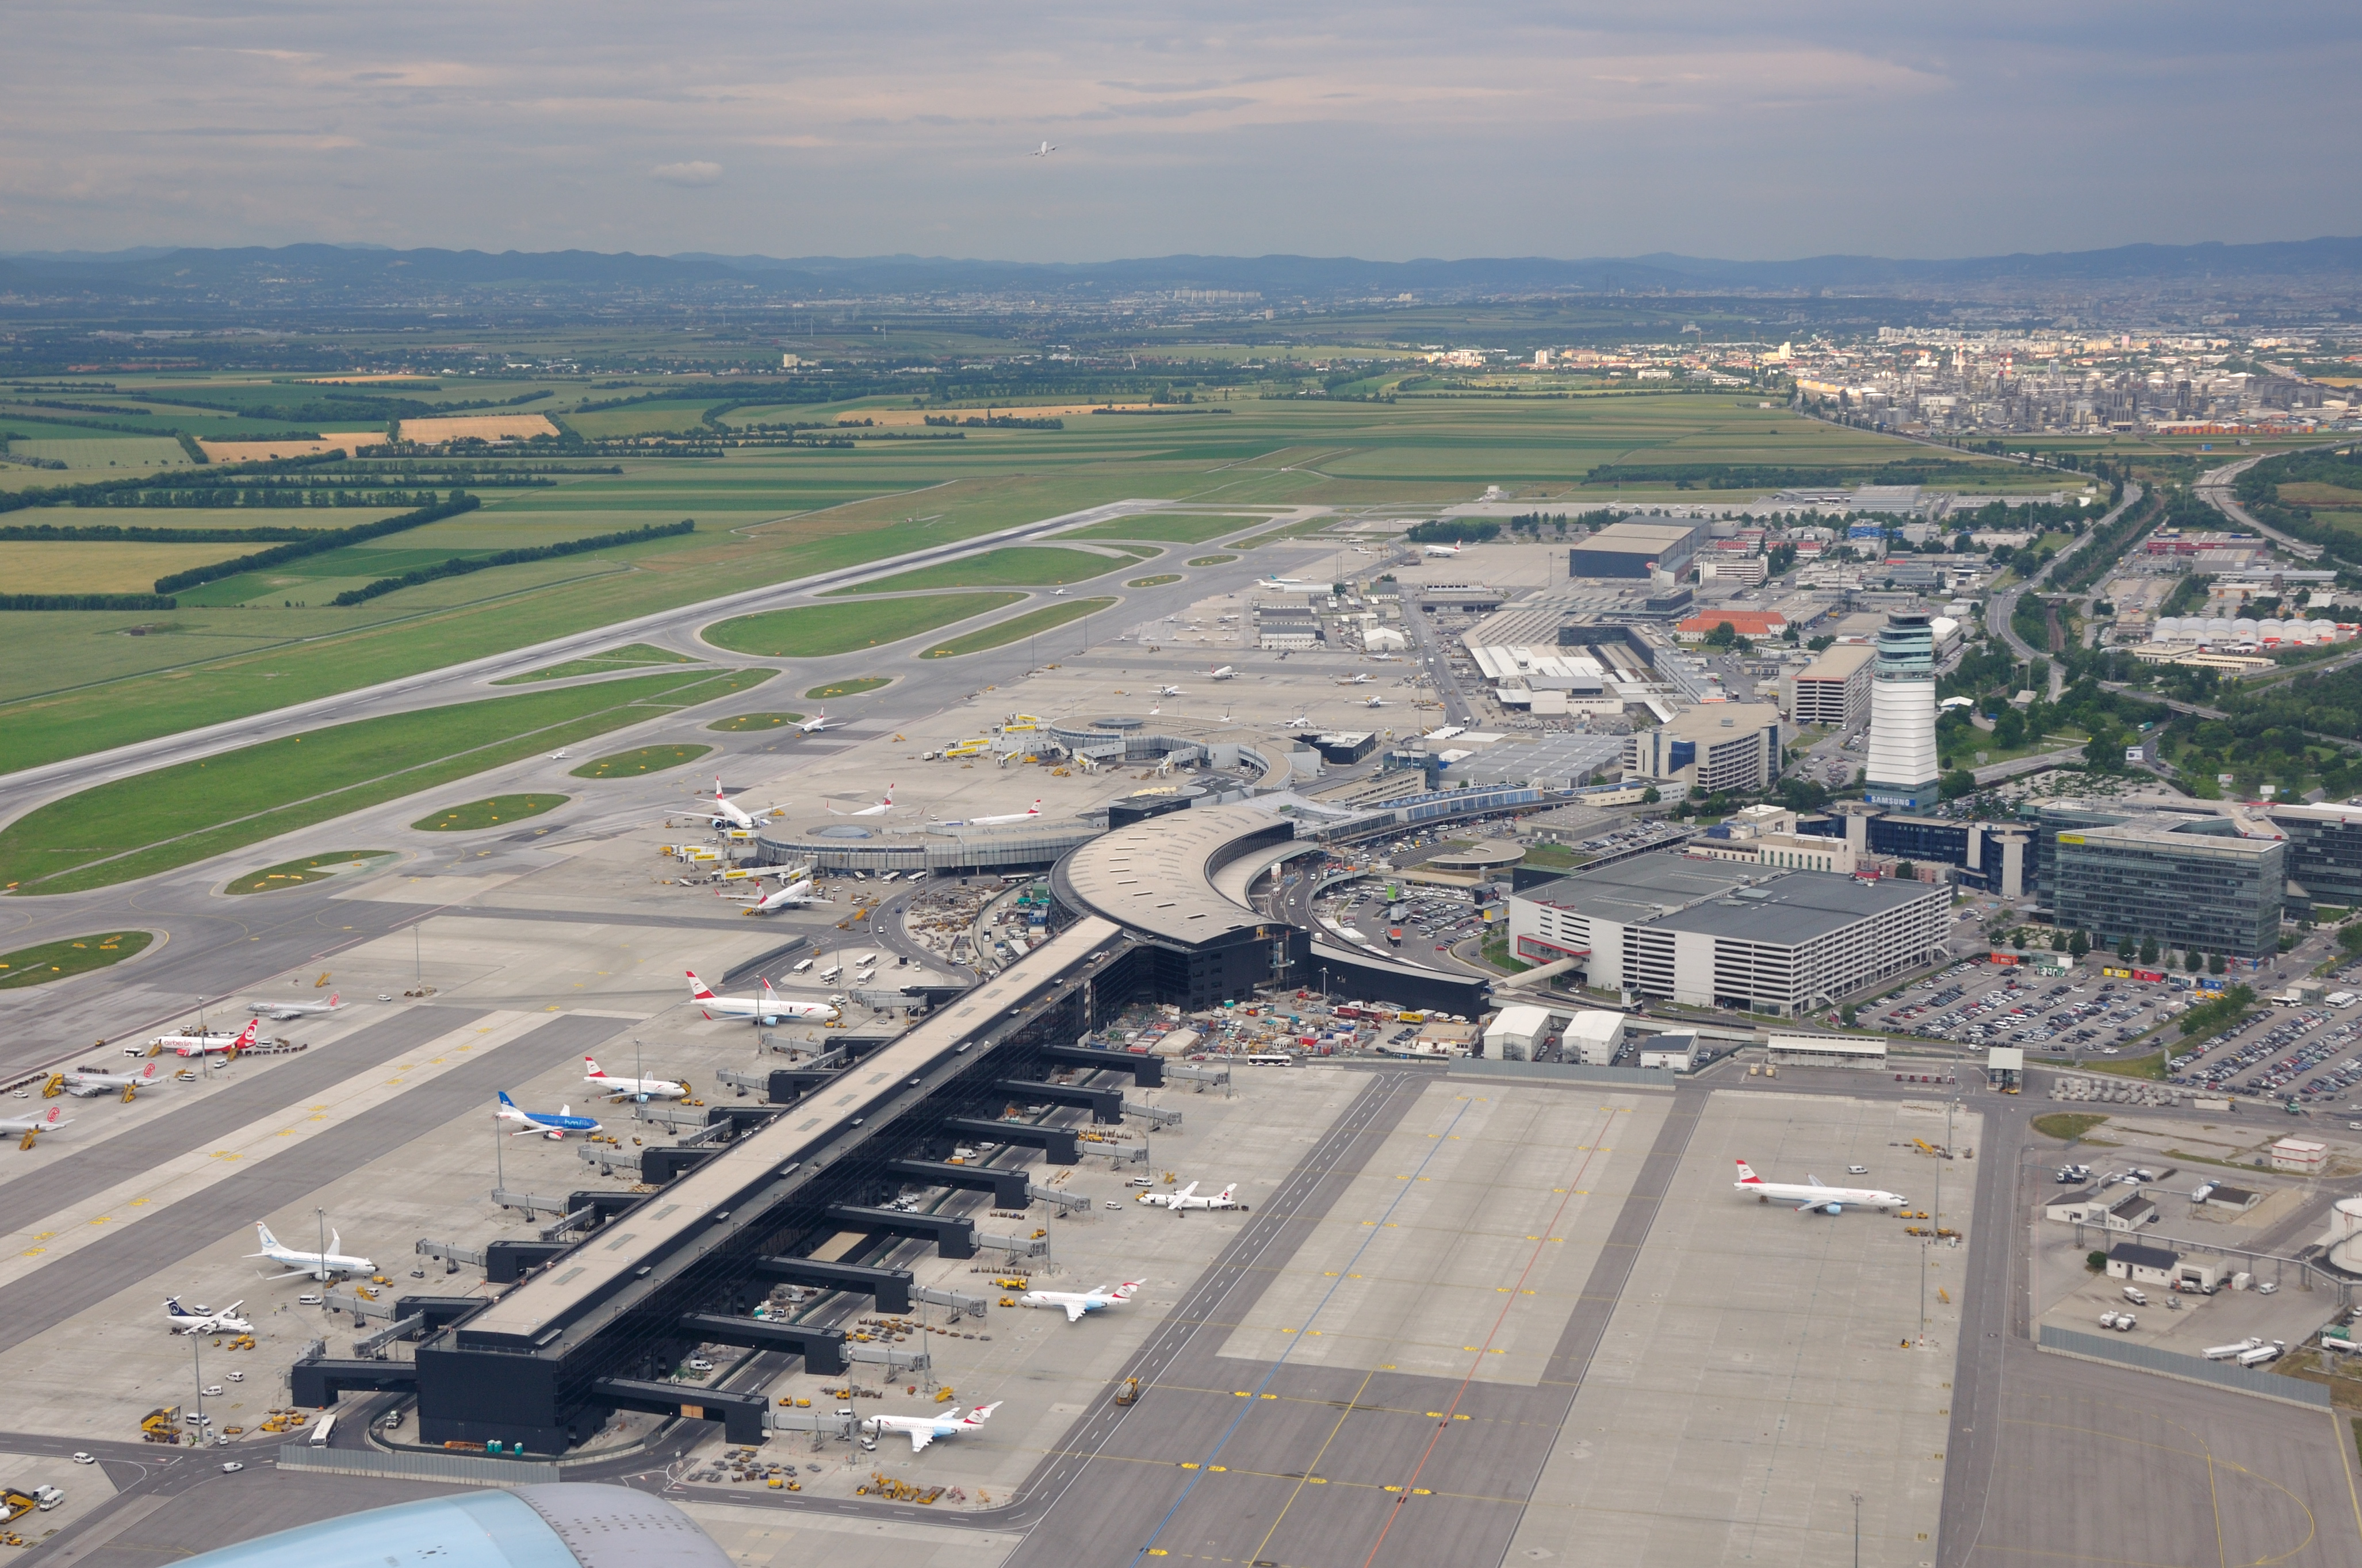
\includegraphics[width=0.7\textwidth]{airport_vienna.jpg}
\footnotesize{Source: Wikipedia}
\end{center}
\end{figure}

\subsubsection*{By Train}
Vienna has good train connections to several European cities and train is the fastest and most convenient
means of transportation between big cities in the region. All trains arrive and depart at the main train
station (Wien Hauptbahnhof).
\begin{description}
\item[\color{kdedarker} Bratislava] -- from Bratislava Hlavná Stanica, hourly, 1~hour, 10 \euro{}
\item[\color{kdedarker} Budapest] -- from Budapest-Keleti, every other hour, 2.75~hours, 19 \euro{}
\item[\color{kdedarker} Prague] -- from Prague Main Station, every other hour, 4~hours, 19 \euro{}
\item[\color{kdedarker} Brno] -- from Brno Main Station, every other hour, 1.5~hours, 9 \euro{}
\end{description}

\subsubsection*{By Bus}
Long-distance bus lines to Vienna are operated by the following companies: Flixbus, Eurolines, StudentAgency (from/to Czech Republic),
Orangeways (from/to Hungary), Polskibus (from/to Poland). If booked in advance, these can offer a cheap alternative to trains or flights.

\subsubsection*{By Car}
Vienna is well-connected to other cities by highways. You can get easily to neighboring countries by car.
Travel time examples:

\begin{description}
\item[\color{kdedarker} Berlin] -- 640 km, 6.75 hours
\item[\color{kdedarker} Budapest] -- 243 km, 2.5 hours
\item[\color{kdedarker} Bratislava] -- 80 km, 1 hour
\item[\color{kdedarker} Prague] -- 300 km, 3.5 hours
\item[\color{kdedarker} Brno] -- 134 km, 1.75 hours
\item[\color{kdedarker} Ljubljana] -- 384 km, 3.75 hours
\item[\color{kdedarker} Zagreb] -- 373 km, 4 hours
\end{description}

Parking near the venue and in most inner districts is not free and only possible for short term. We recommend to park either at your accomodation or in a Park \& Ride garage (Cost: 17 \euro{} for one week).

\subsubsection*{How to get around}
Viennas big public transport system consists of 5 subway lines, tramways, busses and a suburban rail network. The following public transport is reachable in a maximum of 10 minutes walking distance: 
\begin{itemize}
	\item 2 subway stations, Karlsplatz (subway U1, U2, U4) and Taubstummengasse (subway U1) 
	\item Trams \#{1}, \#{2}, \#{62}, \#{71} and D
	\item Bus 59A
\end{itemize}

\vspace{10pt}
Ticket prices (valid for the whole city): 
\begin{itemize}
	\item Single ride: 2,20 \euro{}
	\item 24 hours: 7,60 \euro{}
	\item 48 hours: 13,30 \euro{}
	\item 8 days (do not have to be consecutive): 38,40 \euro{}
	\item Week ticket (Monday till Monday): 16,20 \euro{}
\end{itemize}

\cleardoublepage

\section*{Conference T-Shirts}
\addcontentsline{toc}{section}{Conference T-Shirts}
Due to the cheaper production costs, we will print the T-Shirts in Slovakia or Czechia. Our first choice would be the Slovakian printing company that did the Akademy 2014 T-Shirts and our second choice would be \url{http://www.t4u.cz/en/}. With both companies the maximum cost per T-Shirt (for around 300 t-shirts) should be 4 \euro{}

\cleardoublepage

\section*{The Venue}
\addcontentsline{toc}{section}{The Venue}
The proposed Venue would be the Technical University of Vienna (TU Wien). TU Wien consists of over 10 indivdual buildings, with most of them clustered in the area around Karlsplatz. Out of those buildings, one of them (Neues EI) would be a good fit for Akademy. Another building (Freihaus) would be a backup option, especially for the BoF days. The location has good public transport connection (see section ''How To Get Around'').\\
Fachschaft Informatik would reserve the necessary rooms, so there would be no reservation fee for them.

\subsection*{Neues EI}
\addcontentsline{toc}{subsection}{Neues EI}

Neues EI (''new electrical-engineering institute'') is a recently renovated building located 10 minutes walking from the subway station Karlsplatz and 5 minutes walking from the subway station Taubstummengasse. Apart from four big lecture rooms on the ground floor, there is a big aula in the building and two areas for computers, that can be used as hacking area for over 100 people. Additionally the building has a small courtyard directly next to the lecture rooms. For Akademy this would be the preferred location due to it being more representative, the simple building layout and easy to find rooms.

\vspace{10pt}

\begin{wrapfigure}{r}{0.5\textwidth}
\vspace{-22pt}
\begin{center}
\includegraphics[width=0.5\textwidth]{neues_ei_tuwien.jpg}
\footnotesize{Neues EI (Source: TU Wien)}
\end{center}
\vspace{-16pt}
\end{wrapfigure}

Conference \& General Assembly rooms:
\begin{description}
\item[\color{kdedarker} EI7] -- 434 seats, one of the biggest \& most representative lecture rooms at TU Wien.
\item[\color{kdedarker} EI8] -- 139 seats, a lecture room located next to EI7.
\item[\color{kdedarker} EI9] -- 181 seats, a lecture room located around the corner of EI7.
\item[\color{kdedarker} EI10]-- 375 seats, a lecutre room located next to EI9.
\end{description}

\vspace{10pt}
\begin{center}
	\includegraphics[width=0.5\textwidth]{EI7_tuwien.jpg}
	\footnotesize{EI7 (Source: TU Wien)}
\end{center}
\vspace{10pt}

For the BoFs, the following rooms can be used:\\
\begin{itemize}
	\item The 4 lecture rooms from above
	\item An additional lecture room in the 3rd floor
	\item Up to 8 seminar rooms on the 2nd to 4th floor
\end{itemize}

\subsubsection*{Equipment}
\addcontentsline{toc}{subsubsection}{Equipment}
All lecture \& seminar rooms are equipped with:
\begin{itemize}
	\item a projector,
	\item a cable to connect a laptop to the projector,
	\item audio (hands-free microphones),
	\item video and audio recording,
	\item wifi connection (encrypted, guest accounts would need to be organized)
\end{itemize}

The entire building is covered by a wireless network.

\subsubsection*{Catering \& nearby Restaurants}
\addcontentsline{toc}{subsubsection}{Catering \& nearby Restaurants}
Under the week (during the BoF days \& the AGM) the main student mensa (located 5 minutes walking distance away), a small buffet directly at the venue and many nearby restaurants are open.\\
For the weekend the following catering options exist:
\begin{description}
\item[\color{kdedarker} Nearby restaurants] While there are a lot restaurants nearby, not all of them are open on the weekend. Additionally they don't offer cheaper lunch menus on weekend.
\item[\color{kdedarker} Mensa Catering] The Mensa of the TU Wien also offers catering. Alternatively they can be asked to open the main mensa and offer 2 menus.
\item[\color{kdedarker} Blue Orange Catering] Blue Orange is a cafe near TU Wien offering bagels \& sandwiches. They offer mixed boxes of 7 different bagels for 38 \euro{} per box.
\item[\color{kdedarker} Pizza Catering] Near TU Wien there are many pizzerias that offer delivery. This can also be comined with catering from Blue Orange.
\item[\color{kdedarker} Water \& SoftDrinks] Vienna has a very good quality tap water. This can be offered for free. Fachschaft Informatik can provide us with crates of cheap soft-drinks that the info-stand can sell. Alternatively Fachschaft Informatik can sell drinks for their standard price.
\end{description}

\newpage

\section*{Social Events}
\addcontentsline{toc}{section}{Social Events}
Vienna offers venues in different styles \& sizes. We already organized different events from student parties at the unversity to big parties with concerts \& DJs.
We will split this section into three sections: Locations for a pre-registration event on Friday, Locations for an Akademy party and ideas for the day trip.


\subsection*{Pre-Registration Event}
\addcontentsline{toc}{subsection}{Pre-Registration Event}

\begin{description}
\item[\color{kdedarker} Nelson's] This is a cafe in the main building of TU Wien. It can be rented for a price of 130 \euro{} for groups bigger than 70 persons. They can also offer Catering.
\item[\color{kdedarker} Fachschaft Architektur \& Informatik] Fachschaft Architektur has a bar and adjacent to it another big room directly in the main building of TU Wien. If the weather is nice, they also have outside seating. Alone or together with Fachschaft Informatik, they can offer us their space, drinks and maybe food for a low price.
\item[\color{kdedarker} Kontaktraum \& Terrace] On the 6th floor of Neues EI is an event location with an adjacent big terrace. The room has space for 90 people. A food catering can be organized or a BBQ on the terrace can be possible.
\item[\color{kdedarker} Metalab] The biggest hackerspace of Vienna also regularly organizes events. They have a cheap bar and space for around 100 people. And they can show people around their hackerspace (althoug this might not be as fancy as a tour through C-Base).
\item[\color{kdedarker} Tunnel Vienna] Tunnel is a student which has space for over 100 people and have good and affordable food.
\end{description}

\subsection*{Akademy Party}
\addcontentsline{toc}{subsection}{Akademy Party}


\begin{description}
\item[\color{kdedarker} Derwisch] Turkish restaurant located at Viennas partystreet (Gürtel). They have a cellar with it's own bar, which can be rented exclusively for around 100 \euro{} or possibly even free. In the cellar music a DJ can play. For the number of people expected, we can get them to offer a free buffet of cold turkish specialities. 
\item[\color{kdedarker} Replugged] Venue for up to 250 people with 2 floors. The lower floor has a stage for concerts. Can be reserved exlusively, free if a certain amount of income from the drinks was made. Only required to pay for a security guard \& technician for a DJ or band.
\item[color{kdedarker} Weberknecht] Bar \& Concert location consisting of 3 floors. Two of them can be rented for a cheap rent or a minimum amount of drink income.
\end{description}

As an alternative, many bars with outdoor space (e.g. at Donau or Donaukanal) exist and thus can on nice \& warm days offer enough space. Some can also be reserved exclusively and a DJ could play there (or music from a laptop or mobile phone could be played).


\subsection*{Day trip}
\addcontentsline{toc}{subsection}{Day trip}
\begin{description}
\item[\color{kdedarker} Kahlenberg Bus trip \& Heurigen Visit] Kahlenberg is a hill in the north-west of Vienna, which offers a scenic panaroma look over the city. Every 15 minutes a Wiener Linien bus (standard ticket price) goes all the way up to the hill. On the hill there is a cafe, a small church \& 2 free terraces with view over the city. After enjoying the views, people can walk down an easy path to Kahlenbergdorf. There we can go to a Heurigen (typical Austrian wine-tavern) or food \& drinks.
\item[\color{kdedarker} Donauinsel BBQ \& Swimming] On Donauinsel, there are big BBQ places to rent for 10 \euro{}. We need to bring coal to make a fire \& people can bring their own food \& drinks. People can bring games to play or can go swimming in the New Danube. Later in the evening, a bonfire can be made using the firewood that the city provides.
\item[\color{kdedarker} Trip to Bratislava] Hop on the train for one hour and be in the capital of another country? Where food \& drinks cost only half the price of Vienna? With a train ticket for just 15 \euro{} (round-trip ticket including public transport in Bratislava) this is possible from Vienna. Bratislava has a castle with view over the city, a small but nice old-town and many big restaurants.
\end{description}

\cleardoublepage

\section*{Accomodation}
\addcontentsline{toc}{section}{Accomodation}
We'd like to provide several price levels of accommodation to suit all conference attendants:

\subsection*{Low Cost}
\addcontentsline{toc}{subsection}{Low Cost}
\begin{itemize}
\item \emph{A \& O Hostel Hauptbahnhof} is a very big Hostel located close to the main train station of Vienna. They have space for at least 200 people in single- \& double-rooms. The price (without a possible discount) is 30 \euro{} per night \& person in a twin room and 50 \euro{} per night \& person in a single room. The rooms have a private toilet \& bathroom. Due to their location, price \& possibility to host nearly all attendees at the Hostel we recommend them as main Hostel. They also have common areas which can be used for late-night hacking. Using public transport it is one subway stop or 25 minutes walking distance to the conference venue.
\item \emph{Wombats Naschmarkt} is a modern \& well-located (12 minutes walking distance from the Venue) hostel. They offer 22 private double rooms for 30 \euro{} per person \& night. The rooms have a private toilet \& bathroom. They are smaller but a bit more centrally located than A \& O, but don't offer the anemnities of the close-by train station (late shopping, direct connection from/to the airport). We recommend them for the team or other people who want to stay longer in Vienna.
\item The \emph{Dorm room in Hotel Grand Ferdinand}  is a room for 8 person for 35 \euro{} per night. Grand Ferdinand is a 5-Star hotel located on the Ringstrasse around the first district. If someone ever wanted to stay in a 5-Star hotel, this is an affordable way to do so :)
\end{itemize}

\subsection*{Mid-Range}
\addcontentsline{toc}{subsection}{Mid-Range}
\begin{itemize}
\item \emph{Motel One Wien Hauptbahnhof} is a modern hotel near the main trainstation. Their rooms start at 70 \euro{} for one person and 85 \euro{} for two persons.
\item \emph{Other Hotels near Hauptbahnhof} are also in this price range. They are all in 10 minutes walking distance of the subway station Hauptbahnhof: Novum Hotel Congress, Star Inn Hotel Premium, Hotel Zeitgeist and Hotel Schani.
\end{itemize}

\section*{Acknowledgements}
\addcontentsline{toc}{section}{Acknowledgements}

\begin{description}
	\item[\color{kdedarker} Daniel Vrátil] -- for providing us with the LaTeX source of the Akademy 2014 proposal
	\item[\color{kdedarker} Albert Astals Cid \& Aleix Pol] -- for answering quite a few questions about the proposal
\end{description}

\cleardoublepage

\section*{Contact}
\addcontentsline{toc}{section}{Contact}
\Author

\end{document}
